\section{Methods}
\label{sec:methods}

%------------------------------------------------

The structure of this work is threefold.
First, a dataset of university course descriptions is generated using publicly available data from a number of North American universities.
This process is discussed in \sref{sec:data-acquisition}.
Second, \ac{lda} is applied to the collected data and topics are inferred.
This step is discussed in \sref{sec:topic-modeling}.
Finally, the collected data and inferred topics are presented in a user-facing web application, described in \sref{sec:visualization}.

%------------------------------------------------

\subsection{Data Acquisition}
\label{sec:data-acquisition}

%------------------------------------------------

The primary data manipulated in this study are university catalog course descriptions.
The current experimental data sources are described in \tref{tbl:dataset}.
Note that only Computer Science departments are included in this dataset, in order to simplify the evaluation process and the required number of inferred topics.
Simple web scrapers were written using Python and BeautifulSoup to download publicly available descriptions from university catalogs.
These will be made publicly available at \url{http://github.com/jrouly/trajectory}.
Descriptions and catalog webpages appear in a vast variety of different formats, structures, and HTML correctness, so a parser was written for each university to acquire the unstructured text.
This text was then passed through a cleaning procedure to remove abbreviations and non-English characters, as well as common English stop words.
Finally the text was passed through a stemmer to strip morphology from the words and eliminate duplicate terms.
At the same time, departmental course prerequisite data is collected from the catalog as well.
Prerequisites are limited to courses in the database, meaning that references older courses that are no longer present in the catalog are ignored.
Non-specific prerequisite references (eg.\ \texttt{400-level}) are ignored as well.

%------------------------------------------------

\begin{table}
  \centering
  \begin{tabular}{lcl}
    \toprule
    University & Course Count \\
    \midrule
    American University & 32 \\
    George Mason University & 145 \\
    Kansas State University & 83 \\
    Louisiana State University & 59 \\
    Portland State University & 190 \\
    Rensselaer Polytechnic Institute & 61 \\
    University of South Carolina & 64 \\
    Stanford University & 69 \\
    University of Utah & 142 \\
    University of Tennessee, Knoxville & 29 \\
    \midrule
    ACM Exemplar Courses & 68 \\
    \bottomrule
  \end{tabular}
  \caption{CS program statistics\label{tbl:dataset}}
\end{table}

%------------------------------------------------

The Python scraping framework developed is structured to allow pluggable web scrapers tooled to specific syllabus repositories.
There are a number of existing web scrapers in place pointing to different university course catalogs, but the code can be easily extended in the future to grow the data set.
Integrated in the scraping framework is a lightweight relational database layer to store both course description data and university metadata, including names, URLs, and prerequisite information.
The database layer also stores inferred topics.

%------------------------------------------------

\subsection{Preliminary Data Exploration}
\label{sec:data-exploration}

%------------------------------------------------

In addition to \ac{lda}, other unsupervised machine learning tools can be applied to the same data set.
Simple clustering algorithms (eg. K-Means) when given the same bag of words corpus as input act to identify groupings of similar documents according to their term frequency vector Euclidean distance.~\cite{lloyd1982}
Additional, similar clustering algorithms can be applied in a similar manner.

%------------------------------------------------

Preliminary exploratory results are promising.
We applied K-Means clustering to a sample dataset of syllabi scraped just from the GMU Computer Science online archive of syllabi.
Using course sections across semesters as ground-truth labels, we obtained metrics summarized in \tref{table:cluster-metrics}.
A distributed implementation of K-Means available in the Python toolkit \texttt{scikit-learn} was used to perform the clustering.

%------------------------------------------------

The high completeness values are promising: this indicates that many of the same course are assigned under the same cluster prototype.
The low value of homogeneity is unsurprising given the initialization parameters used: K-Means was initialized to detect only 20 clusters, a far smaller number than the magnitude of distinct course sections available.
The number 20 was chosen arbitrarily as a smaller count than the true number of distinct course sections in order to increase cluster size.
Cursory visual inspection of the most common frequencies in the first few clusters also supports the structured nature of the dataset with related terms grouped together in a logical fashion corresponding with an obvious, known GMU course.

%------------------------------------------------

\begin{table}[ht]
\centering
\begin{tabular}{ll}
\toprule
Execution time & 0.144568s \\
Homogeneity & 0.415 \\
Completeness & 0.877 \\
V-measure & 0.563 \\
\bottomrule
\end{tabular}
\caption{Preliminary clustering metrics\label{table:cluster-metrics}}
\end{table}

%------------------------------------------------

\subsection{Topic Modeling}
\label{sec:topic-modeling}

After the exploratory clustering process, we pass\-ed clean\-ed data into a topic modeling framework by exporting from the database layer to the filesystem in a structured ``bucket of files'' format.
The Java MALLET library is used to perform \ac{lda} on the course description data.
A data pipeline is constructed using the MALLET API that reads input data, tokenizes it, and trains an \ac{lda} topic model.
The inferred topics are then exported to a common \ac{csv} format and read back into the database layer and applied to existing courses.
Independent runs of \ac{lda} with distinct parameterization are segregated in the database into ``Result Sets'', allowing sets of inferred topics to sit side by side without interfering.
This also allows the presentation of different sets of inferred topics to the end user.

%------------------------------------------------

The initialization parameters of MALLET's \ac{lda} implementation are summarized in \tref{table:lda-parameters}.
Experiments were run varying parameters throughout the experimental range, including the MALLET default values.
However, as the number of topics increased greatly beyond 750, and as $\beta$ decreased greatly below 0.0001, the MALLET framework began to encounter instability and errors.
Any runs which encountered infinite or ``not-a-number'' values were immediately discarded.
Ultimately 77 result sets were retained for analysis.

%------------------------------------------------

\begin{table*}[ht]
\centering
\begin{tabular}{llll}
\toprule
Parameter  & Description & Experimental Range & Default \\
\midrule
$\alpha$   & Dirichlet concentration parameter. & [1, Iterations] & Iterations \\
$\beta$    & Dirichlet concentration parameter. & [0.0001, 0.5] & 0.01 \\
Iterations & The number of \ac{lda} iterations. & --- & 3000 \\
Topics     & The number of topics to infer. & [100, 1000] & --- \\
\bottomrule
\end{tabular}
\caption{LDA Initialization Parameters\label{table:lda-parameters}}
\end{table*}

%------------------------------------------------

\subsection{Visualization}
\label{sec:visualization}

%------------------------------------------------

An interactive, dynamic user visualization of course descriptions and topics has been prototyped.
The visualization is a web-based application built upon the Python Flask library.
The tool interfaces with the same database layer used by the rest of the application framework to provide an aesthetically pleasing user-facing interface with several primary modules.
By default, the web application presents the user with a high level ``dashboard'' overview of the dataset and available result sets, where a result set is the set of topics inferred after a single run of the \ac{lda} module with a distinct initialization set.
\fref{fig:dashboard} shows the dashboard view.
After selecting a result set, the user can browse the data by course, department, or university.

%------------------------------------------------

\begin{figure}
  \centering
  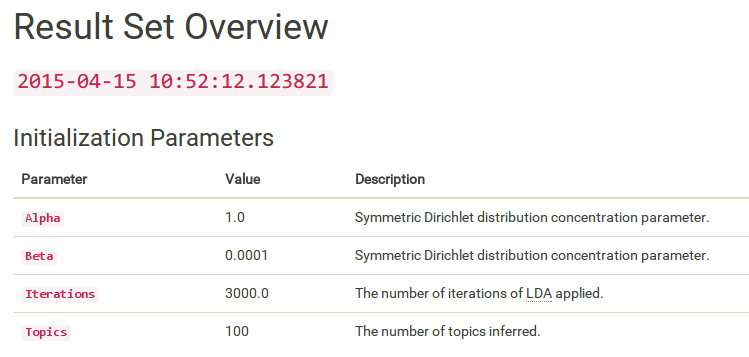
\includegraphics[width=0.45\textwidth]{figures/screenshots/dashboard/result_set_overview.png}
  \caption{Result Set Overview in Dashboard view\label{fig:dashboard}}
\end{figure}

%------------------------------------------------

On selecting a course, the inferred topics are listed in order of their proportion in the course's description.
Additionally, an interactive collapsible tree visualization of the course' prerequisite chain in the department is displayed.
This tree visualization provides a view of the conceptual overlap of courses and prerequisites.
\fref{fig:prerequisite-detail} details the prerequisite tree visualization.

%------------------------------------------------

\begin{figure}
  \centering
  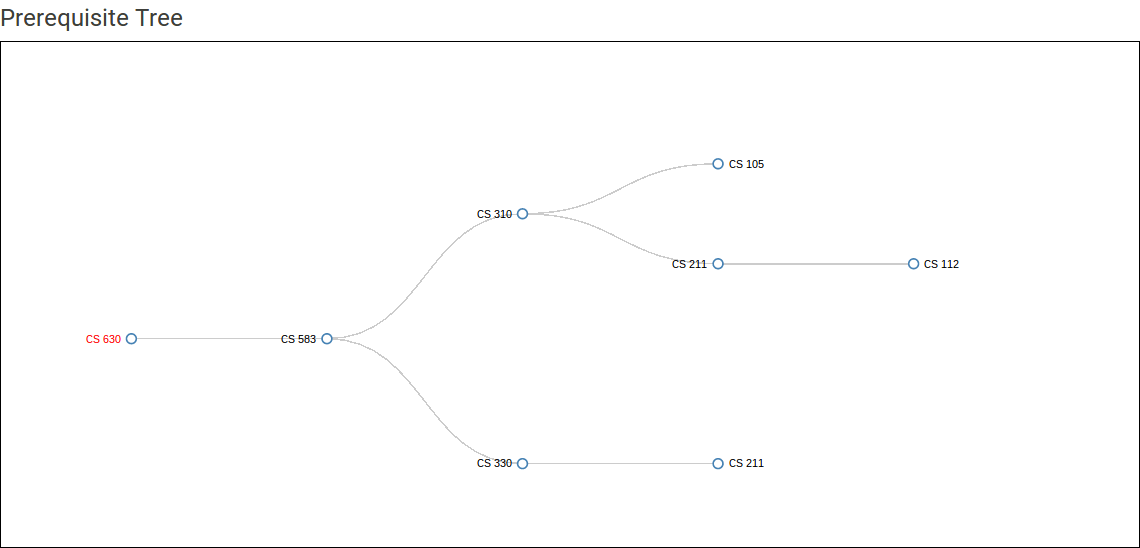
\includegraphics[width=0.45\textwidth]{figures/screenshots/course/prerequisite_detail.png}
  \caption{Interactive prerequisite tree visualization tool\label{fig:prerequisite-detail}}
\end{figure}

%------------------------------------------------

The user may also compare two university departments.
Topics inferred from every course in the department are collected and displayed side by side, along with the intersection set of common topics.
Similarity metrics describing the relationship between the two departments are given as well --- the Jaccard index, cosine similarity, and euclidean distance.
The first metric is based solely on topic set cardinalities, while the remaining are based on a ``topic-vector'' representation of the department.
The topic-vector is a binary vector where each feature indicates whether a particular topic was inferred for the given department.
Features are unweighted as the topic-vector indicates only whether a topic is present in a department's topic set, and not its frequency of occurrence.
See \fref{fig:statistics} for an image of the departmental comparison tool.

%------------------------------------------------

\begin{figure}
  \centering
  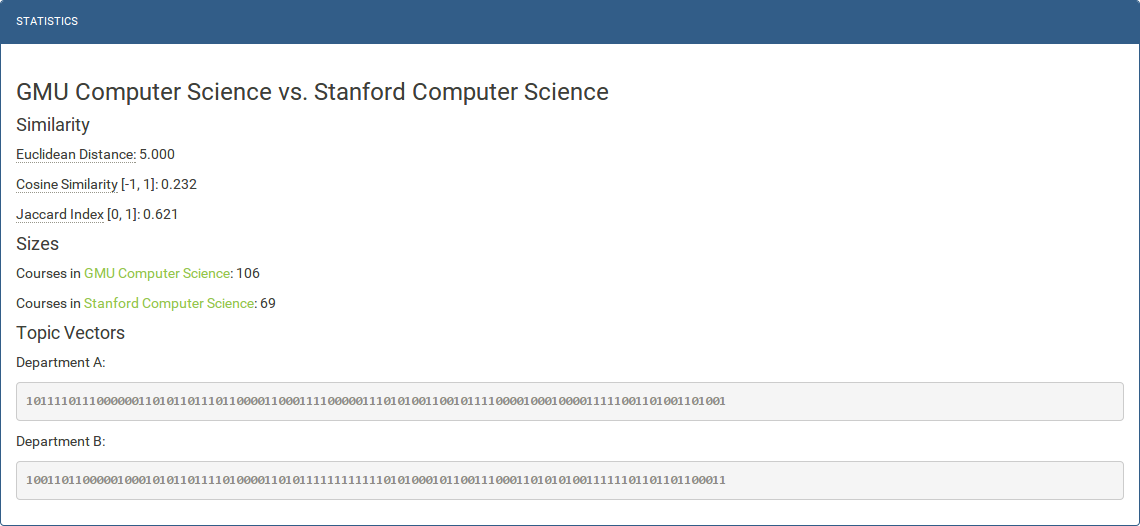
\includegraphics[width=0.45\textwidth]{figures/screenshots/compare/statistics.png}
  \caption{Statistics generated by departmental comparison tool\label{fig:statistics}}
\end{figure}

%------------------------------------------------

Using third party benchmarks discussed in \sref{sec:evaluation}, the tool also allows users to automatically evaluate the performance of a university department.
The tool checks for conceptual overlap between courses and \ac{acm} Knowledge Areas and predicts Knowledge Area labels where overlap exists.
Then, using manually annotated ground truth labels, the tool evaluates its performance by measuring the similarity between prediction and truth label sets.
\fref{fig:evaluation} shows the evaluation tool in use.

%------------------------------------------------

\begin{figure}
  \centering
  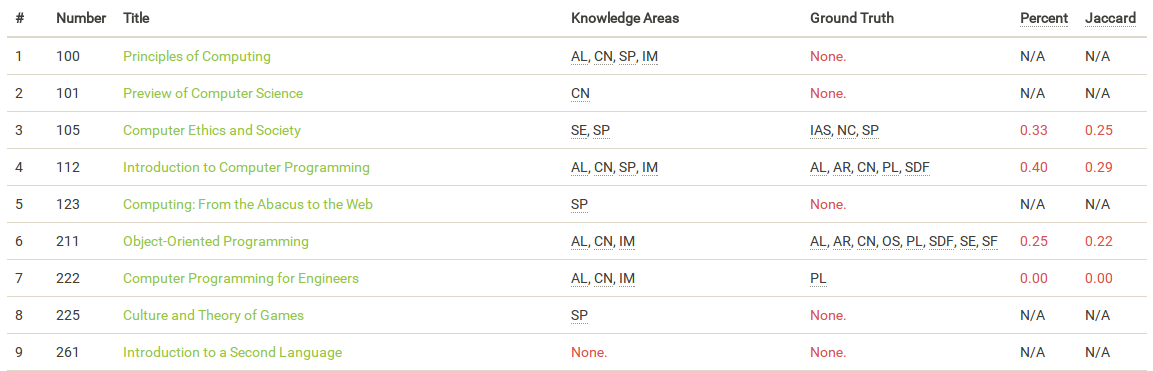
\includegraphics[width=0.45\textwidth]{figures/screenshots/evaluate/evaluation.png}
  \caption{Evaluation tool in use\label{fig:evaluation}}
\end{figure}

%------------------------------------------------
